\itemhead{p.76 练习 · 第1题（教材p.76）}{XJ-B1-C03-PR-P076-Y0217}
\label{XJ-B1-C03-PR-P076-Y0217}
{\footnotesize 湘教版教材p.76 / PDF第83页 / p.76 练习 / 第1题}
\field{原题}{作出下列函数的图象，并写出函数的值域：
\subq{1}$y=|x+3|$；
\subq{2}$y=|x-2|-|x+2|$。}
\field{参考答案}{（1）顶点 $(-3,0)$ 的V形图，值域 $[0,+\infty)$；（2）$f(x)=4$（$x\le-2$）、$-2x$（$-2<x<2$）、$-4$（$x\ge2$），值域 $[-4,4]$。}
\begin{center}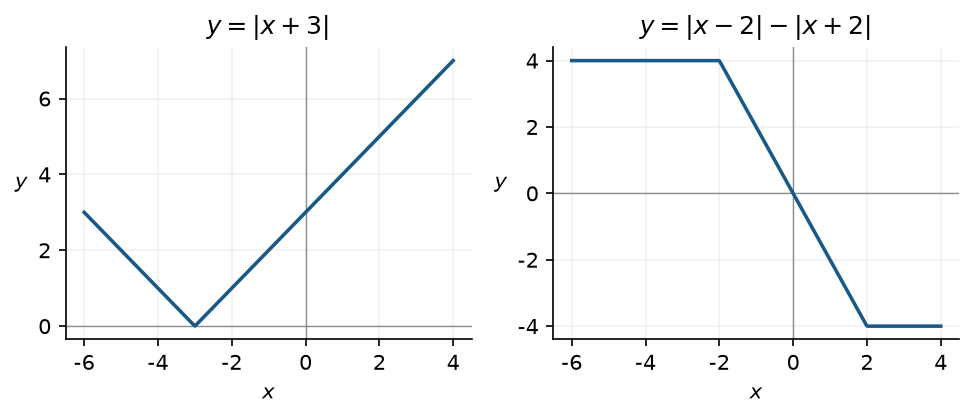
\includegraphics[width=.84\linewidth,height=.38\textheight,keepaspectratio]{figures/C03-PR076-1.png}\end{center}
{\small \field{关联知识}{F07 分段函数、绝对值及分段应用（教材帮p.86、91、92、93 / PDF95、100、101、102）；F04 函数三种表示法、图象与读数（教材帮p.85、86、93、94 / PDF94、95、102、103）}
\field{方法与易错点}{先列转折点和各段条件，再建立分段式，检查衔接、定义域与值域。 易错：跨段套公式；超额部分按全量收费；绝对值去号漏区间。}
\field{答案依据}{答案册相关题组：PDF第20页（册内页19）；按当前题库原题逐项重算，不按旧版题号机械对套。}}
